\raggedright
\setlength{\parindent}{2em} %首行缩进
\newpage


\setcounter{section}{1}


\section{研究計畫內容}

\subsection{摘要}
微笑美學被認為是患者選擇牙科治療的重要原因,因此數位微笑設計(DSD)技術的出現,將幫助矯正醫師更方便診斷分析患者的微笑美學,並向患者視覺化呈現。數位微笑設計技術可以幫助矯正醫師在治療過程中,對患者的牙齒進行模擬,並根據患者的需求和預期效果調整。此外,數位微笑設計還可以提供更加直觀和易于理解的建議,讓患者更清晰地了解矯正過程的全貌。

但是如今的微笑設計軟體仍需要矯正醫師手動標記參考線、牙齒位置等資訊,無法做到軟體自動分析患者微笑美觀構成,因此尚不能做到即時向患者視覺化呈現。因此本研究旨在將實例分割技術應用於微笑設計(DSD),希望透過實例分割模型自動分析微笑照片,分割並標記牙齒、嘴唇、牙齦,最後將分割結果用於計算微笑美觀參數。因為在DSD的應用場景中,主要分析患者正顱與側顱的影像,因此本研究將針對正顱與側顱訓練分割模型。我們會使用AI生成的人臉與向患者搜集的照片作為訓練集,並使用YOLACT++與BlendMask模型進行訓練,最後比較評估兩種模型的辨識結果。本研究計畫假設能在符合DSD臨床使用的情況下,得到更好的分割精度(AP)。該分析模型將用於開發一套易於使用的微笑特徵辨識系統,用以簡化DSD軟體操作流程,幫助矯正醫師及時向患者呈現矯正或是微笑訓練的成果。




 

\newpage
\subsection{研究動機與研究問題}


現今患者越來越意識到有吸引力的微笑對臉部美觀的重要性,因此矯正學除了重視咬合關係外,也開始重視咬合與周圍軟組織的協調性,微笑的吸引力是專業人士評斷審美偏好的重要標準\upcite{smile_importance}。此外,改善面部和牙齒的吸引力亦是患者尋求牙科治療的主因之一。在日常社交互動,微笑對於面部美學有顯著影響\upcite{smile_preferences_of_orthodontists},因此微笑在矯正中是十分重要的。

許多因素都會影響微笑美學,例如,微笑線、牙唇關係、微笑弧度、協調的的面部比例以及對稱性\upcite{frush1958dynesthetic}\upcite{hulsey1970esthetic}\upcite{sarver2007aesthetic}。然而微笑美學是主觀的,受到個人經歷與社會社會環境影響。例如由於牙科經歷不同,矯正牙醫、一般牙醫和非專業人士之間對微笑的偏好存在明顯差異\upcite{smile_preferences_of_orthodontists}\upcite{微笑審美差異}。甚至在不同地區或性別的矯正醫師間仍從在顯著差異\upcite{smile_preferences_of_orthodontists}\upcite{微笑審美差異2}。因此在矯正治療與微笑訓練上,矯正醫師需要考慮患者對微笑的美觀偏好,診斷評估並與患者溝通微笑美觀的各種構成。


若能有效率的分析微笑構成並呈現,將能輔助矯正醫師診斷,並有效降低醫師與患者的溝通成本,而這些正是現今數位微笑設計(DSD,digital smile design)技術的目標\upcite{dsd_tech}\upcite{dsd_tech2}\upcite{charavet2019benefits}。目前的DSD技術主要是紀錄患者前牙列的2D圖像或是面部掃描的3D數據上\upcite{dsd_tech}\upcite{dsd_tech2}\upcite{dsd_tech3d}。但是在影像分析上,仍需要醫師先手動繪製參考線、標記輪廓與形狀,例如面部中線、門牙切線等,軟體方能取得影像或模型的美學參數資訊\upcite{dsd_tech}。

人工智能 (AI) 已經大幅改變我們的生活。尤其是機器學習(ML)技術,得利於其優異的圖像處理和決策支援能力,其在各領域皆有廣泛應用。在醫學影像上,卷積神經網路(CNN)透過學習標記過的醫學影像,已經在診斷視網膜病變\upcite{renita}、間質性肺疾病(Interstitial Lung Disease)\upcite{lung}有良好成效。在口腔矯正領域,卷積神經網路(CNN)影像處理也在2D 頭部x光影像的標註\upcite{cepha_net}、檢測矯正患者牙齦炎的早期徵兆\upcite{gingivitis}方面取得有效成果。

但是對於DSD技術中的二維圖像標註,目前仍須矯正醫師手動進行,並未應用卷積神經網路(CNN)影像辨識。雖然目前已有研究訓練YOLACT++模型分割微笑的二維圖像,但在牙齒的分割上成效不佳\upcite{YOLACT++分割}。該研究是以各種不同角度的微笑圖片進行訓練,而在DSD的使用場景中,分析對象是以固定角度、固定方法拍攝的微笑照片(正顱、側顱)\upcite{dsd_tech}\upcite{dsd_tech2}\upcite{cheng2021relationship}。另外,因為YOLACT++是較重視辨識速度的模型,因此其準確度比起辨識速度較慢的BlendMask模型差\upcite{BlendMask}\upcite{YOLACT++}。所以本研究希望分別利用YOLACT++與BlendMask模型,針對不同角度(正顱、側顱)分別重新訓練微笑圖像的實例分割模型,並評估比較其辨識效果,希望能提升各辨識目標精度(AP)的分割模型。最後開發一套易於使用自動微笑特徵辨識系統,將辨識結果用以輔助醫師與患者溝通微笑構成與評估微笑訓練成效。



\subsection{文獻回顧與探討}
\subsubsection{微笑的美觀構成}

關於研究中微笑的美觀構成,目前已經有許多論文對微笑的構造提出數種美觀參數以量化,並透過問卷調查得知不同族群對這些參數的偏好\upcite{smile_preferences_of_orthodontists}\upcite{微笑審美差異}\upcite{微笑審美差異2},例如在Pasukdee等人的研究中探討了矯正醫師、一般牙醫師、矯正患者、一般大眾分別對數個美觀參數的偏好,其中包含\upcite{smile_preferences_of_orthodontists}:\\




\begin{figure}[H]
\centering
\includegraphics[width=0.8\textwidth]{paste_src/2023-02-05-22-20-04.png}
\caption{微笑美觀參數定義\upcite{smile_preferences_of_orthodontists}}
\label{}
\end{figure}

這些美觀參數多可從患者的正面、側面的微笑影相中獲得,為了自動辨識這些參數,本研究希望能透過深度學習模型,自動從微笑照片中的分割以下特徵:鼻子、上唇、下唇、各顆牙齒、牙齦與Buccal corridor



\subsubsection{DSD軟體}

根據Coachman等人的研究,將會拍攝患者正面、側面照片用作DSD分析\upcite{dsd_tech2}。而在Jafri 等人的研究中,他們操作了現今常見的12種DSD軟體,認為這些軟體確實能幫助面部美學視覺化。他們不僅能幫助患者了解治療結果,也能幫助醫師診斷與治療\upcite{dsd_tech}。但是這些軟體仍需要臨床醫師標註參考線、牙齒位置等,仍不能自動分析微笑美觀構成。

\begin{figure}[H]
\centering
\begin{minipage}[b]{0.4\textwidth} %minipage寬
\centering
\includegraphics[width=1\textwidth]{paste_src/2023-02-07-20-49-33.png}
\caption{正面照\upcite{dsd_tech2}}
\label{fig:正面}
\end{minipage}
\begin{minipage}[b]{0.4\textwidth} %minipage宽
\centering
\includegraphics[width=1\textwidth]{paste_src/2023-02-07-20-50-39.png}
\caption{側面照\upcite{dsd_tech2}}
\label{fig:側面}
\end{minipage}
\end{figure}


\begin{figure}[H]
\centering
\includegraphics[width=1\textwidth]{paste_src/2023-02-07-21-26-21.png}
\caption{DSD軟體操作介面\upcite{dsd_tech}}
\label{}
\end{figure}

\subsubsection{實例分割}
在實例分割研究上經典的Mask R-CNN模型是基於檢測框的雙階段算法,在訓練與辨識皆需要等待檢測框\upcite{mask_r-cnn}。而在單階段算法上,YOLACT模型移除了localization step 來加速,實現實時實例分割(Real-time Instance Segmentation),但精度較差\upcite{YOLACT}。而YOLACT++是在YOLACT算法的基礎上改善精度,根據Bolya等人的研究結果,YOLACT++可在COCO資料集取得33.5fps 下獲得34.1mAP的成績。而跟據Chen等的研究成果,BlendMask模型相較於YOLACT雖然速度較慢,但提升了精度,在ResNet-101骨架下能在COCO資料集取得37.8的AP值\upcite{BlendMask}。

\begin{figure}[H]
  \centering
\includegraphics[width=.5\textwidth]{paste_src/2023-02-06-20-56-24.png}

  \caption{各模型在COCO資料及的測試結果\upcite{YOLACT++}}

\end{figure}


\begin{figure}[H]
\centering
\includegraphics[width=1\textwidth]{paste_src/2023-02-06-20-58-26.png}\caption{BlendMask在COCO資料集的測試結果\upcite{BlendMask}}
\label{}
\end{figure}



在Lee \& Kim(2022)的研究\upcite{YOLACT++分割} 中,使用NVIDIA公司發布的Flickr-Faces-HQ (FFHQ)資料集的5500張圖片進行訓練,其中包含各種角度的成人臉孔。並對眼睛、眉、鼻子、上唇、下唇、耳屏、牙齦、頰走廊、各顆牙齒  標註。在實例分割模型選擇上,他們使用YOLACT++架構,基於ResNet-101骨架和FPN。最後對每個特徵的辨識結果計算平均精度(AP)以定量評價模型品質。其中平均精度(AP)是透過 精確率–召回率曲線得到,綜合考慮精度、召回率、IoU得到的指標。最後在IoU域值0.5下得到在眼睛、鼻子、嘴唇都獲得高於0.9的AP值,在t13-t23的牙齒範圍取得80\%以上的準確率。以下為其成果演示:



\begin{figure}[H]
\centering
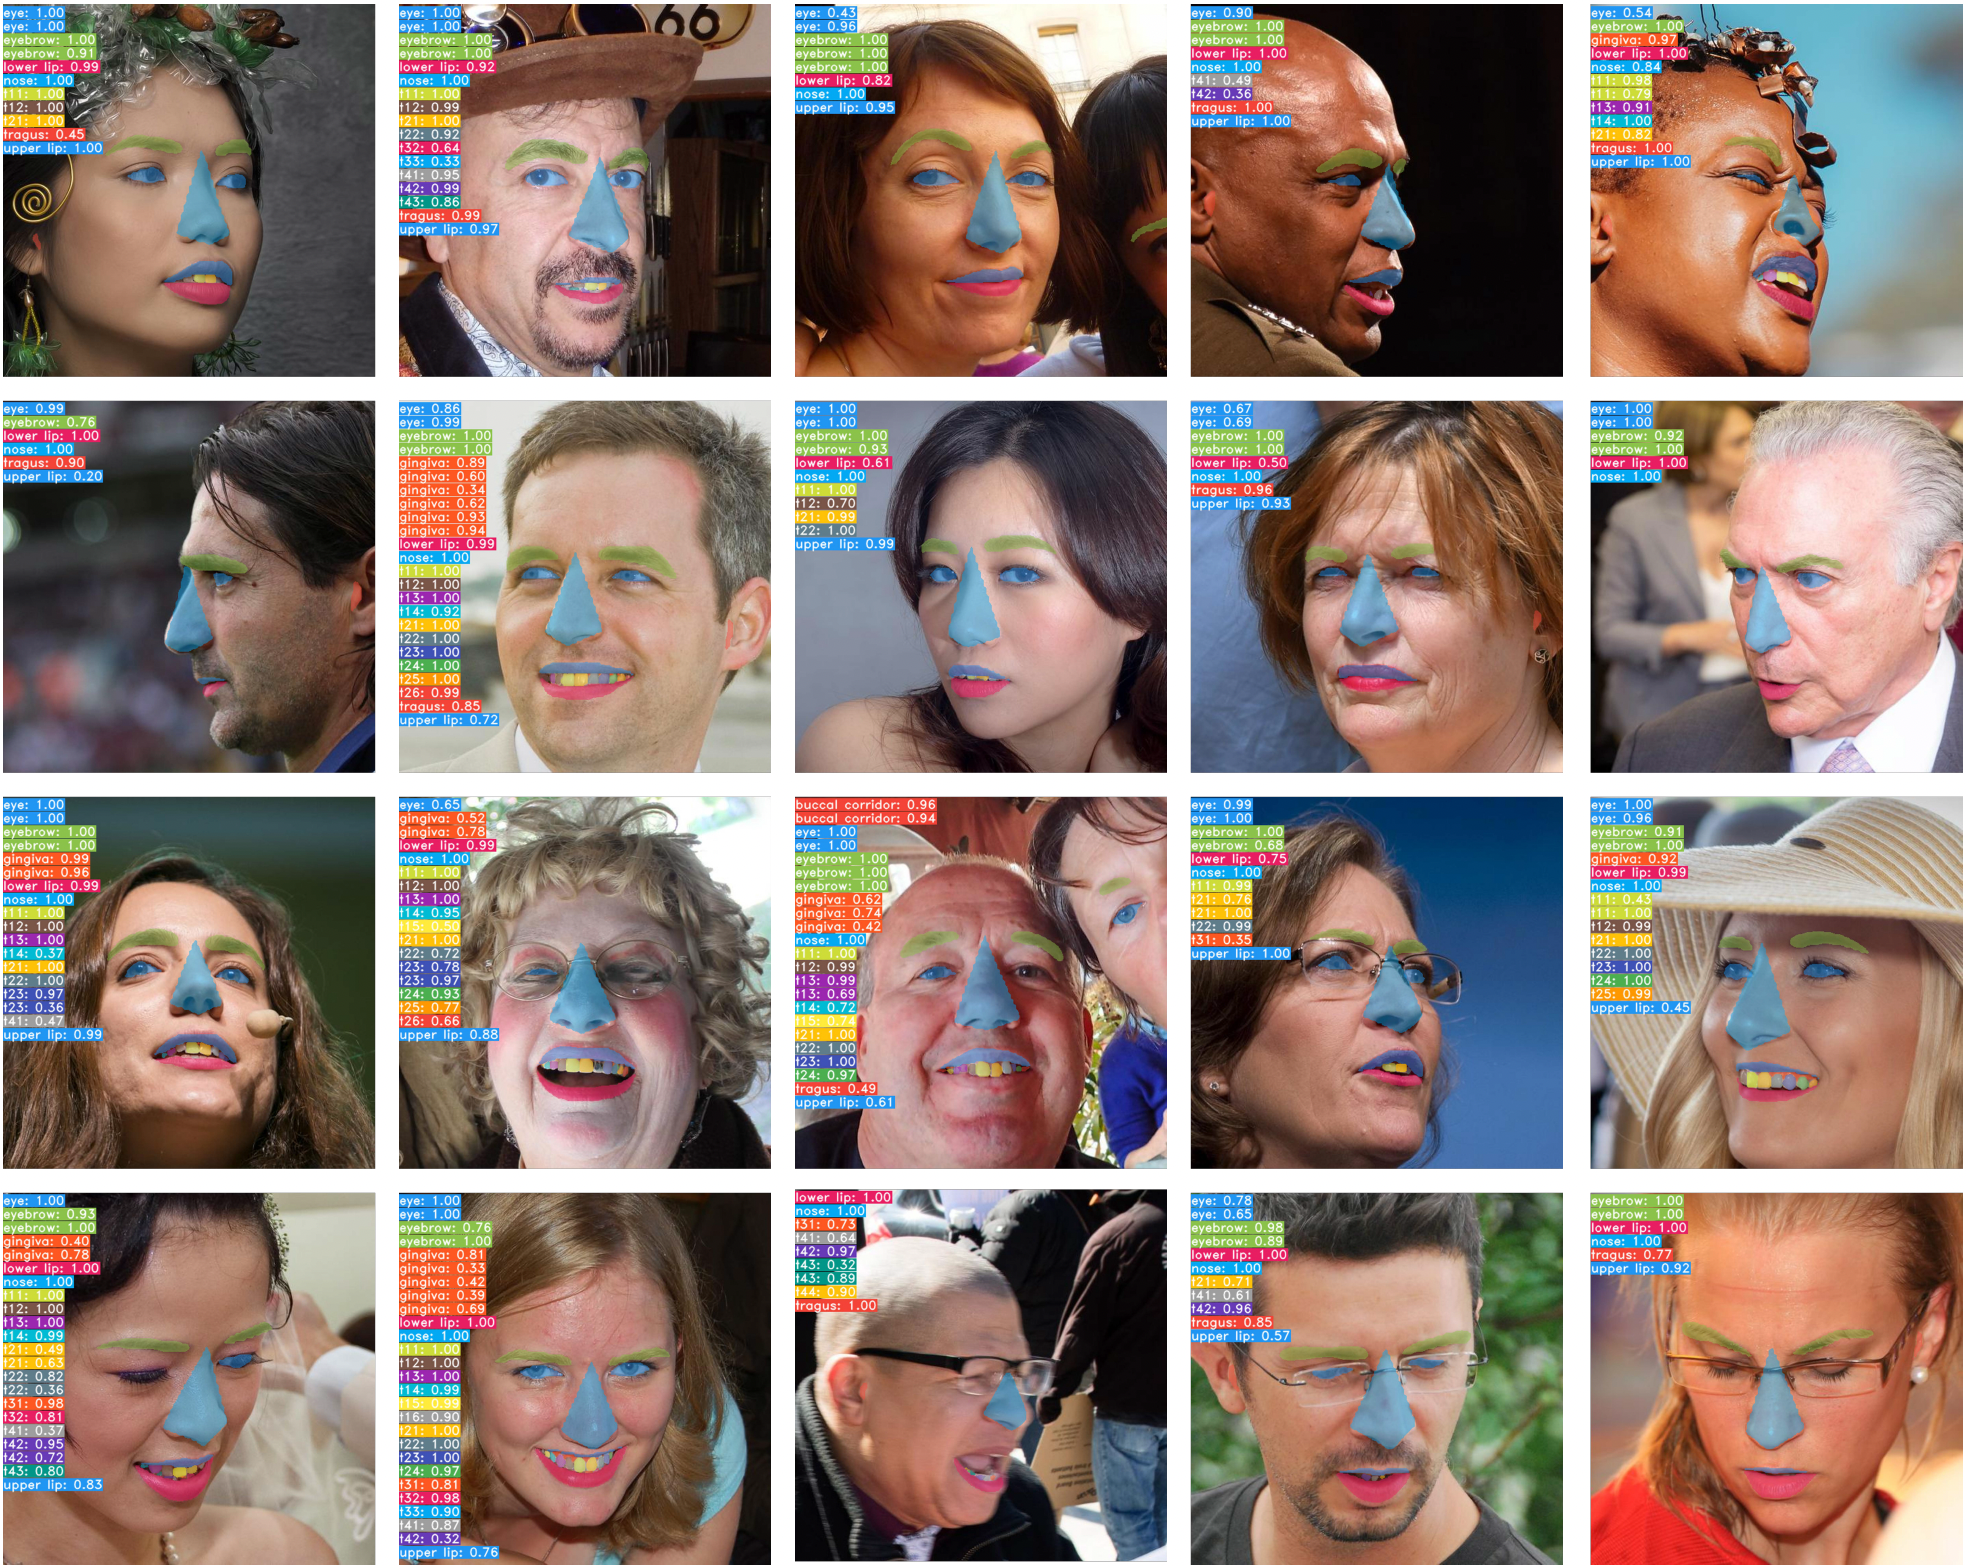
\includegraphics[width=0.7\textwidth]{paste_src/2023-02-06-14-42-37.png}
\caption{YOLACT++分割結果\upcite{YOLACT++分割}}
\label{}
\end{figure}

\begin{figure}[H]
  \centering
  \includegraphics[width=1\textwidth]{paste_src/2023-02-07-22-15-13.png}
  \caption{Lee \& Kim(2022)訓練的模型AP值\upcite{YOLACT++分割}}
  \label{fig:rt}
  \end{figure}


這說明了基於YOLACT++的實例分割模型確實能在微笑美觀構成之圖像分割上取得良好效果。但是因為Lee \& Kim的訓練資料是各個角度的人臉照片,牙齒的資訊較少,所以在牙齒的分個效果較差(如\prettyref{fig:rt},在IoU閾值0.5下,辨識框與分割的AP值分別0.604, 0.411)。但是在DSD的使用場景中,2D圖像的微笑分析對象是固定角度拍攝的,而且比起辨識的速度,更關心辨識的精準度\upcite{dsd_tech}\upcite{dsd_tech2}。因此本研究希望只使用固定角度的微笑影像進行訓練,並且比較 BlendMask 模型與YOLACT++模型的精度(AP),本研究計畫假設能在符合DSD臨床使用的情況下,得到好的辨識效果。




\subsection{研究方法及步驟}

\subsubsection{數據集準備}
微笑照片的來源分為兩部分,首先是向患者搜集,再來是使用AI生成的人臉照片(來自https://generated.photos/ 或是 https://this-person-does-not-exist.com/)。




\begin{figure}[H]
\centering
  \includegraphics[width=.8\textwidth]{paste_src/2023-02-07-18-59-47.png}
\caption{generated.photos生成的人臉}
\label{}
\end{figure}

\newpage
\subsubsection{數據標註}
將使用Labelme 以多邊形標註待辨識的特徵。其中包含:上嘴唇、下嘴唇、各顆牙齒、牙齦和Buccal corridor。

\begin{figure}[H]
  \centering
  \includegraphics[width=1\textwidth]{paste_src/2023-02-07-19-16-30.png}
  \caption{使用labelme標註,照片來自https://this-person-does-not-exist.com/ 生成}
  \label{}
\end{figure}


\subsubsection{模型訓練}
研究中使用的BlendMask模型與YOLACT++模型都是透過python3, pytorch 10.0.1, Detectron2實現。而CNN模型訓練通常不會從頭開始訓練,否則訓練時間太長且需要的資料集過大,因此從他人訓練好的權重開始訓練。
\begin{itemize}
\item[1)]YOLACT++\\
因為希望獲得較高精度,選擇Resnet101-FPN作為架構(backbone)\upcite{YOLACT++}。根據YOLACT++原論文作者的github介紹(https://github.com/dbolya/yolact),權重將繼承自作者提供的權重,輸入圖片大小為$550\times 550$。
\begin{figure}[H]
  \centering
  \includegraphics[width=0.75\textwidth]{paste_src/2023-02-06-21-03-31.png}
  \caption{YOLACT++模型\upcite{YOLACT++}}
  \label{}
\end{figure}
\item[2)]BlendMask\\
因為希望獲得較高精度,選擇R\_101\_dcni3\_5x 作為架構(backbone)\upcite{BlendMask}。根據BlendMask原論文作者的github介紹(https://github.com/aim-uofa/AdelaiDet/tree/master/configs/BlendMask),需要使用AdelaiDet在Detectron2執行訓練\upcite{AdelaiDet}。
\end{itemize}






\begin{figure}[H]
\centering
\includegraphics[width=1\textwidth]{paste_src/2023-02-06-21-01-25.png}
\caption{BlendMask模型\upcite{BlendMask}}
\label{}
\end{figure}




\subsubsection{統計評估}
\df IoU\\

\begin{minipage}[b]{0.4\textwidth}
$$
\mbox{IoU}=\frac{\mbox{交集面積}}{\mbox{連集面積}}
$$
\hspace*{\fill}
\hspace*{\fill}
\end{minipage}
\begin{minipage}[b]{.4\textwidth}
  \includegraphics[width=1\textwidth]{paste_src/2023-02-06-23-34-01.png}

\end{minipage}

\df 精確率(Precision)、召回率(Recall)\\
若以信度大於95\%作為閾值,$\mbox{IoU}>0.5$作為正確(True):\\


\begin{tabular}[t]{|c|c|c|}
\hline
 &  信度大於0.95的辨識框 & 信信度不大於0.95的辨識框 \\
\hline
$\mbox{IoU}>0.5$ & TP   & FP \\
$\mbox{IoU}\leq 0.5$  & FN   & TN \\
\hline
\end{tabular}
\hspace*{\fill}
$$
Precision=\frac{TP}{TP+FP}\ ,
\ \ 
Recall=\frac{TP}{TP+FN}
$$


\df 精度(AP)

將辨識出來的候選框依信度由高至低依序作為信度閾值,可得到一系列精確率、召回率。繪製精確率-召回率圖形(\prettyref{fig:pr}藍線)即可由曲線下面積得到。在計算時會使用橘色線($P_{smooth}$)近似。
$$
AP=\int_{0}^{1}P_{smooth}(r) dr
$$
\begin{figure}[H]
  \centering
  \includegraphics[width=0.7\textwidth,height=6cm]{paste_src/2023-02-07-15-35-26.png}
  \caption{精確率-召會率圖}
  \label{fig:pr}
\end{figure}

\subsection{預期結果}
\subsubsection{分割模型}
我們將會針對正面與側面照(如\prettyref{fig:正面},\prettyref{fig:側面}),使用YOLACT++ 和 BlendMask 算法訓練實例分割模型,並比較分析其辨識結果。希望能比Lee, Seulgi \& Kim, Jong-Eun 得到更好的精度(AP)\upcite{YOLACT++分割}

\subsubsection{微笑分析系統}

在完成模型後,我們希望開發一套手機拍照後即可自動對微笑照片進行分割,再計算相關美觀參數的系統。該系統將使用Python 與 Flask 在伺服器架設api,用戶拍照後即上傳照片到伺服器分析。該系統將用於即時向患者視覺化呈現微笑訓練、矯正的結果,也能輔助醫師進行診斷與治療。


\begin{figure}[!htp]
  \centering
  \begin{tikzpicture}[node distance=2cm]

  \node (start) [startstop] {用戶透過手機app或是網頁拍攝微笑照片};
  \node (input1) [process,below of=start] {照片上傳伺服器};
  \node (process1) [process,below of=input1] {伺服器即時自動分析微笑照片};
  \node (out) [startstop,below of=process1] {將分析結果回傳到手機};


  \draw [arrow] (start) -- (input1);
  \draw [arrow] (input1) -- (process1);
  \draw [arrow] (process1) -- (out);


  \end{tikzpicture}
\end{figure}


\subsection{需要指導教授指導內容}

\subsubsection{微笑照片的搜集}
我沒有搜集醫學資料的經驗,對於該如何搜集資料與搜集資料該注意的問題,如該如何取得患者同意等,我並不熟悉。因此在搜集微笑照片上,需要指導教授的協助。
\subsubsection{臨床知識}
因為本計畫目標將辨識成果應用在臨床上,但臨床知識是我所缺乏的。因此這方面需要指導教授的幫助,指導我怎麼樣的使用情境是臨床上需要的,而我又該達到怎麼樣的辨識精度或該實現怎麼樣的功能。

hi

\bibliography{bibfile} 
\bibliographystyle{unsrt}
